%!TEX ROOT=ctutest.tex
\chapter{Vibrační signály a jejich digitální zpracování}

    Vibrační analýza je samotnou podstatou celé práce. Tato kapitola se snaží vysvětlit původ vibračního signálu a techniky jeho zpracování.

\section{Poruchy indukčních motorů}
\label{section:poruchy_mororu}
    K selhání motorů může dojít mnoha způsoby. Může se jednat o poškození vinutí statoru, defekt rotoru, ale statistika ukazuje, že 40 až 90 \% poruch je zapříčiněno defektem ložisek \cite{book:1}, jejichž původ může být různého druhu, jak ukazuje následující seznam \cite{prez:1}.
    \begin{figure} [!h]
        \centering
        \caption{Příčiny poruch indukčních motorů. Převzato z \cite{prez:2}.}
        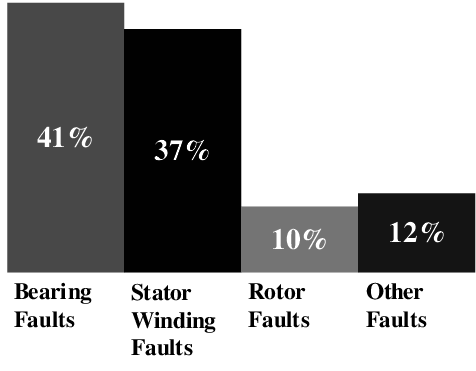
\includegraphics[width=0.4\textwidth]{DSP/Figs/failures.png}
    \end{figure} 
   
    \begin{itemize}
        \item Vady před uvedením do provozu – rozměrové a tvarové nepřesnosti, brusné trhliny.
        \item Vady způsobené nesprávným upevněním k hřídeli – nesouosost, excentricita.
        \item Vady způsobené únavou materiálu ve valivém styku – povrchová styková únava.
        \item Vady způsobené vnějšími vlivy – mazání, znečištění, koroze.
    \end{itemize}
    
    \begin{figure} [!h]
        \centering
        \caption{Příklady poškození ložisek}
        \begin{subfigure}[b]{0.48\textwidth}
             \centering
             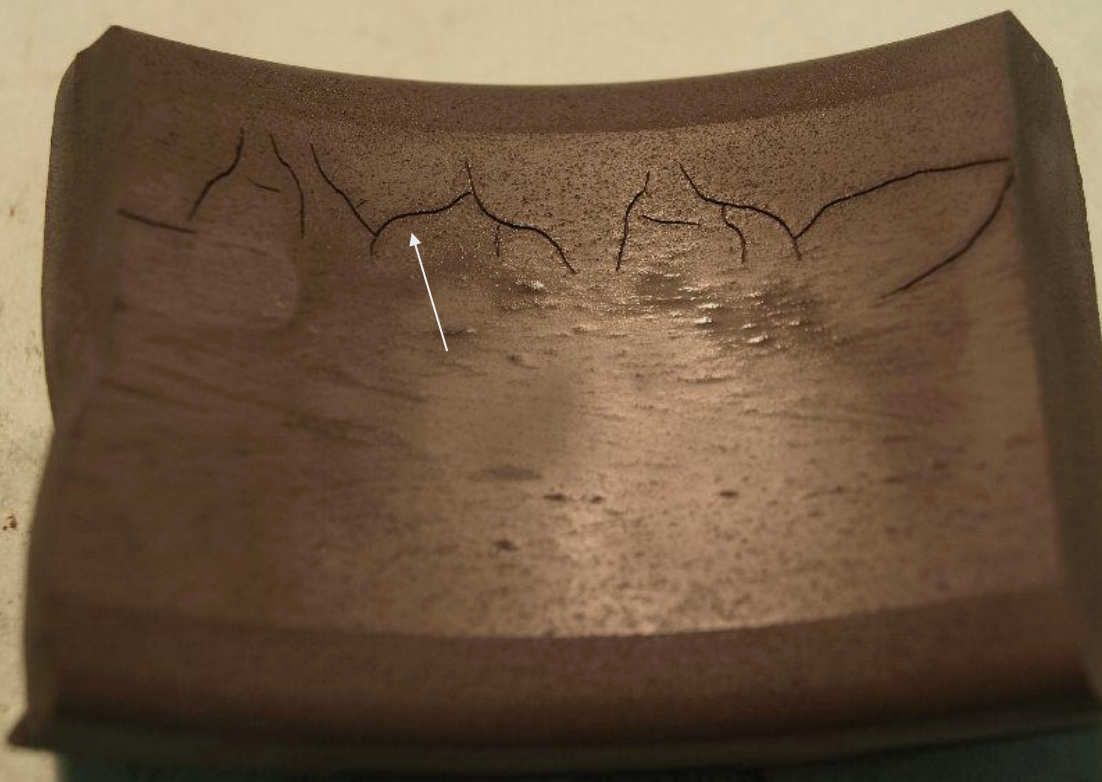
\includegraphics[width=\textwidth]{DSP/Figs/poruchy_lozisek.png}
             \caption {Brusné trhliny na vnitřním kroužku. Převzato z \cite{prez:1}.}
         \end{subfigure}
         \hfill
        \begin{subfigure}[b]{0.46\textwidth}
            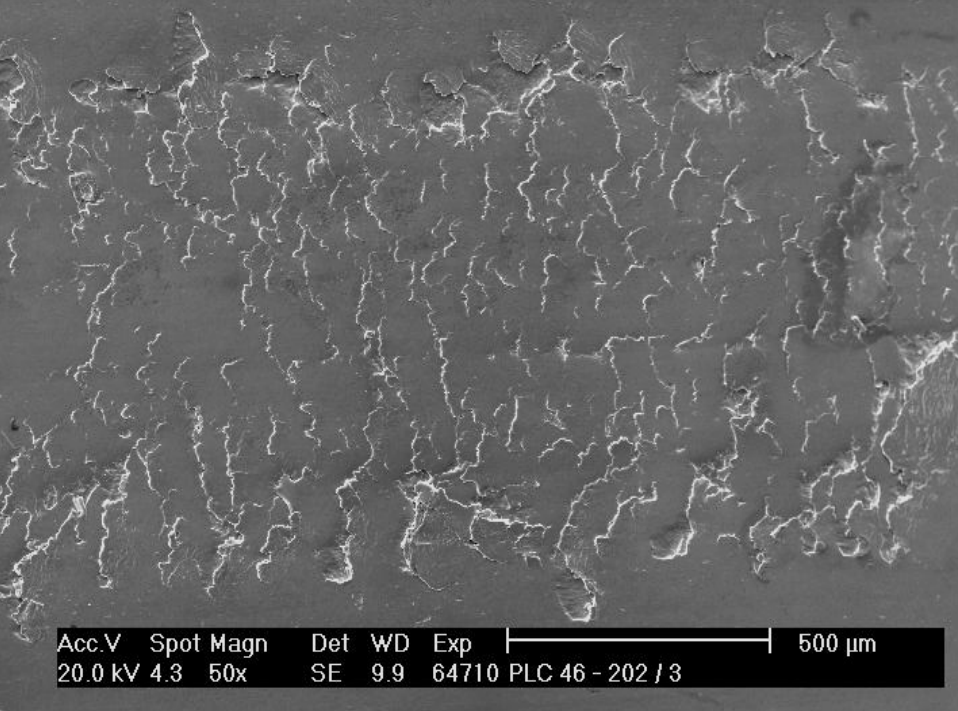
\includegraphics[width=\textwidth]{DSP/Figs/poruchy_lozisek2.png}
            \caption {Povrchové únavové poškození, tzv. pitting. Převzato z \cite{prez:1}.}
        \end{subfigure}
    \end{figure} 
    
    
    
    Analýza vibrací je nejpoužívanější a nejpřínosnější metodou diagnostiky poruch rotačních zařízení \cite{book:1}. Pomocí vibrací lze diagnostikovat poruchu už v~jejím raném stádiu – až měsíce před tím, než dojde k úplnému selhání stroje, což je mnohem dříve než je tomu u ostatních veličin, které lze monitorovat, jako akustických emisí, tepla nebo proudového odběru (viz obrázek \ref{figure:condition}).\\
    Všechna rotační zařízení bez ohledu na dobu provozu a opotřebení vytvářejí vibrace. 
    Vibrační signál motoru v sobě tedy nese velké množství informací, jejichž povaha se navíc po dobu provozu postupně mění. Vlastnosti tohoto signálu jsou determinovány jednotlivými částmi motoru (hřídel, převodovka, turbína, ložiska\ldots) a také v sobě reflektují jeho vady a nedokonalosti.
    Správné porozumění a interpretace těchto vlastností spojená s vhodnými analýzami a technikami zpracování signálu je tedy klíčová pro určení vznikajících poruch při CBM.
    
    \begin{figure} [!h]
        \centering
        \caption{Výhody analýzy vibrací. Převzato z \cite{prez:2}.}
        \label{figure:condition}
        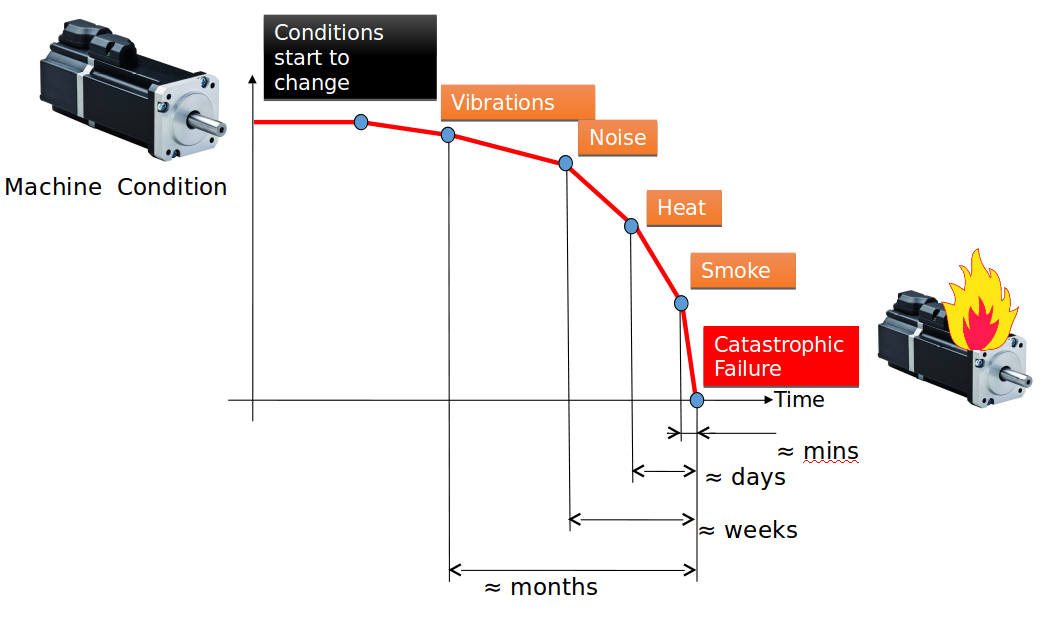
\includegraphics[width=0.8\textwidth]{DSP/Figs/condition.png}
    \end{figure} 

\section{Snímání vibračního signálu}
\label{section:measuring}
    Vibrační signál se získává prostřednictvím měření akcelerace na určitém místě motoru. Kvalita naměřeného signálu silně závisí na umístění akcelerometru v~rámci zařízení. Vibrace lze měřit ve směru osy motoru a ve dvou zbývajících osách kolmých na osu motoru, které bývají pro monitorování důležitější. Můžeme tedy použít jeden trojosý akcelerometr, nebo tři jednoosé. Frekvence signálu se obvykle pohybují od 10 Hz po 10 kHz, jak ukazuje obrázek \ref{figure:vibration}, a jejich konkrétní hodnotu určuje část motoru, ve které vibrace vznikly.
    
    Signál je z akcelerometru přiveden na vstup AD převodníku, jehož vzorkovací frekvence pro splnění Nyquistova teorému musí být alespoň dvakrát větší než maximální frekvence obsažená ve vibračním signálu. 
    \begin{equation}
        f_s \gg 2\,f_{max}
    \end{equation}
    Navržený systém díky konfiguraci, jež lze za běhu aplikace nahrát do měřicí jednotky, umožňuje, aby si uživatel vzorkovací frekvenci sám definoval a upravoval podle konkrétních potřeb, o čemž pojednávají více kapitoly \ref{section:config} a \ref{section:periferie}.
    
     \begin{figure} [!h]
        \centering
        \caption{Typické zdroje vibrací – hřídel, převodovka, turbína a ložiska. Převzato z \cite{prez:2}.}
        \label{figure:vibration}
        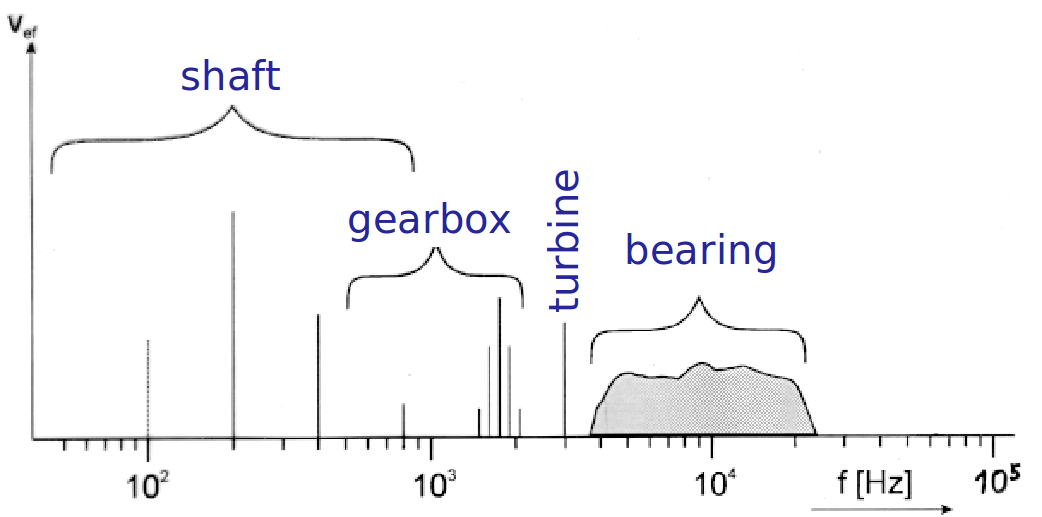
\includegraphics[width=0.85\textwidth]{DSP/Figs/vibrations.png}
    \end{figure} 

    
\section{Techniky zpracování signálu}
\label{section:techniky}
    Mnohé příznaky defektu motoru mohou být určeny přímo v tzv. časové oblasti signálu získaného z akcelerometru. Samotnému zpracování ale obvykle předchází určité předzpracování jako odstranění střední hodnoty a filtrace.\\
    Mocnějším nástrojem jsou poté techniky pracující se signálem ve frekvenční oblasti, které jsou z diagnostického hlediska mnohem komplexnější a poskytují informace o celkovém chování motoru. Motor je ze své podstaty periodické zařízení. Příznaky defektů ložisek se také periodicky opakují, a lze je proto detekovat ve spektru \cite{book:2}. Použití frekvenčních metod je úzce spojeno s~algoritmem FFT (Fast Fourier Transform) umožňujícímu efektivní získání spektra signálu.
    
\subsection{Techniky pracující se signálem v časové oblasti}
    
    \subsubsection{RMS (Root Mean Square)}
    Jednou z nejjednodušších analýz je výpočet efektivní hodnoty, která představuje kvadratický průměr a dobře popisuje celkovou sílu vibrací. Obecně platí, že se její hodnota zvyšuje s otáčkami stroje a pomocí jejího časového trendu dokážeme dobře detekovat větší defekty a opotřebení ložiska.
    \begin{equation}
        u_{RMS} = \sqrt{\frac{1}{N}\sum_{i=1}^{N} u[i]}, 
    \end{equation}
    kde $N$ je počet vzorků a $u_i$ je hodnota $i$-tého vzorku.
    
    
     \subsubsection{Krest faktor}
     \label{section:krest}
        Krest faktor je robustnější technika podávající informaci o impulsivnosti signálu. Obdélníkový nebo stejnosměrný signál má krest faktor roven jedné.\\
        Čím je tedy krest faktor vyšší, tím je signál impulsivnější. U běžných vibračních signálů motorů se krest faktor pohybuje mezi 2 a 6. Vyšší hodnoty obvykle indikují ostré nárazy uvnitř ložiska nebo motoru a obdobně jako u~RMS má krest faktor největší přínos při sledování jeho časového trendu.
        \begin{figure} [!h]
            \centering
            \caption{Časový průběh krest faktoru vzhledem ke změnám efektivní a maximální hodnoty napětí. Převzato z \cite{book:1}.}
            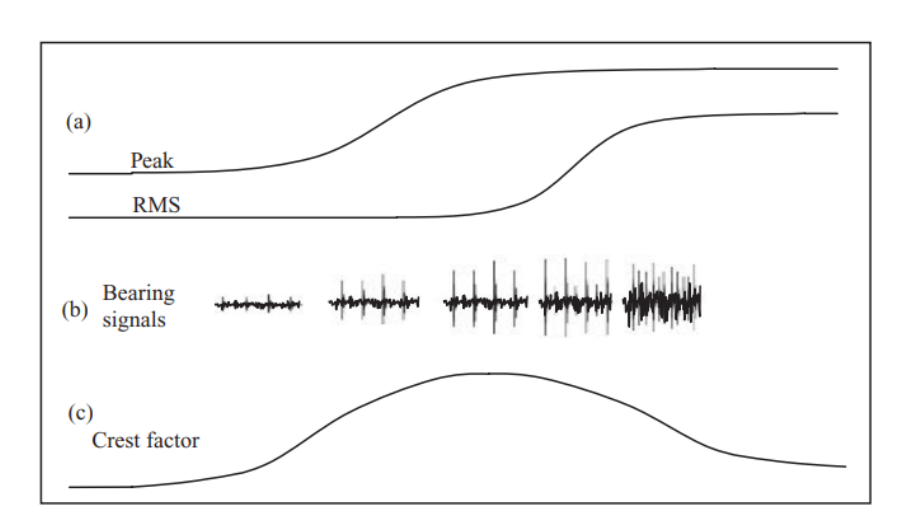
\includegraphics[width=0.8\textwidth]{DSP/Figs/krest_factor.png}
        \end{figure} 
        
        \begin{equation}
            CREST = \frac{|u_m|}{u_{RMS}}, 
        \end{equation}
        kde $u_m$ je maximální hodnota signálu a $u_{RMS}$ je efektivní hodnota.
  

    \subsubsection{Statistické momenty a Kurtosis Ratio}
    \label{section:kurtosis}
        Statistický moment je jednou z charakteristik pravděpodobnostního rozdělení. První a druhý moment je označován jako střední hodnota a variace, čtvrtý jako kurtosis (česky koeficient špičatosti). Pro vibrační analýzu je nejvýznamnější právě čtvrtý moment. Obecně platí, že nepoškozené ložisko vykazuje hodnoty kurtosis kolem 3, což odpovídá normálnímu rozdělení. Vyšší hodnoty poté mohou indikovat vadu \cite{book:2}.
        \begin{align}
            \mu = \text{E}\left[X\right] = \frac{1}{N}\sum_{i=1}^{N} x[i]\\
            \text{VAR}\left[X\right] = \sigma^2 = \text{E}\left[\left(X - \mu\right)^2\right]\\
            \text{KURT}\left[X\right] = \text{E}\left[\left(\frac{X - \mu}{\sigma}\right)^4\right]
        \end{align}
        
        Kurtosis Ratio je poté technika vyjadřující množství odchylek v signálu v~čase.
        Signál se nejprve ořízne, odstraní se z něj vychýlené hodnoty, tedy 5-10~\% největších a nejmenších hodnot (tato hodnota je přesně určena konfiguračním parametrem \texttt{dsp\_kurtosis\_trimmed\_samples}, více v kapitole \ref{section:config}) a spočítá se jeho kurtosis. Výsledkem je poté poměr kurtosis neoříznutého a oříznutého signálu. Pro signály, jež nevykazují vychýlené hodnoty (typicky obdélníkový signál), je kurtosis i po oříznutí stejná, a výsledek je tedy roven jedné \cite{article:2}.
        
        \begin{figure} [!h]
            \centering
            \caption{Oříznutí signálu pro výpočet kurtosis ratio. Převzato z \cite{article:2}.}
            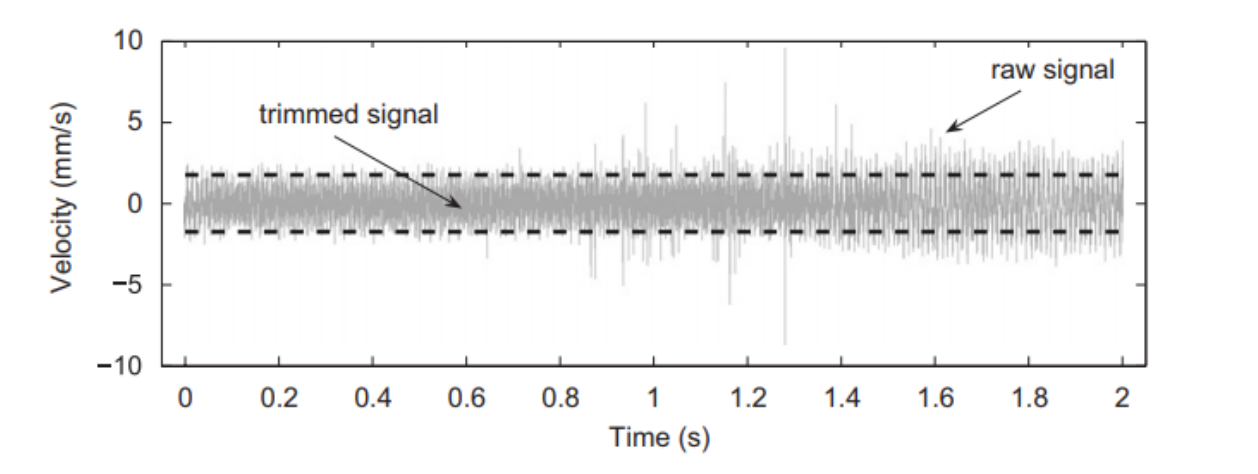
\includegraphics[width=\textwidth]{DSP/Figs/kurtosis_ratio.png}
        \end{figure} 
        
    \subsubsection{Starší, výpočetně nenáročné techniky}
        
        Následující tři techniky pocházejí z dávné minulosti, kdy AD převodníky nedosahovaly takových vzorkovacích frekvencí jako dnes a k zpracování signálu byl použit komparátor a čítač. Dnes se ale stále používají zejména u analýz velmi rychlých signálů jako jsou akustické emise s kmitočty kolem 10-1000~kHz. Především díky jejich výpočetní nenáročnosti a stále zajímavému informačnímu charakteru, který je v navržené aplikaci umocněn konfigurovatelností jejich parametrů – napěťové úrovně (konfigurační parametr \texttt{dsp\_voltage\_threshold}, více v kapitole \ref{section:config}), jsme se rozhodli, aby byly použity i v naší aplikaci pro analýzu vibrací.\\
        Jedná se konkrétně o tyto techniky, jejichž význam lze dobře vidět na obrázku \ref{figure:burst}.
       
        \begin{enumerate}
            \item \textbf{Ringdown Counts} – počet průchodů signálu předem určenou komparační napěťovou úrovní.
            \item \textbf{Rise Time} – doba náběhu signálu od prvního průchodu napěťovou úrovní po maximální hodnotu.
            \item \textbf{Signal Duration} – doba od prvního průchodu napěťovou úrovní po poslední průchod.
        \end{enumerate}{}
        
        \begin{figure} [!h]
            \centering
            \caption{Grafické znázornění technik využívajících komparační napěťovou úroveň. Převzato z \cite{website:8}.}
            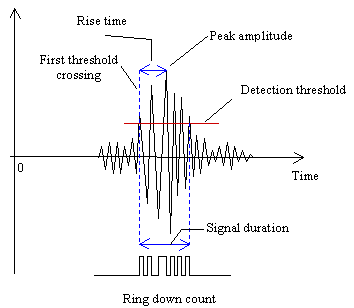
\includegraphics[width=0.8\textwidth]{DSP/Figs/burst.png}
            \label{figure:burst}
        \end{figure} 
        
        
    \subsection{Techniky pracující se signálem ve frekvenční oblasti}
    \subsubsection{FFT – amplitudové spektrum}
        Diskrétní Fourierova transformace signálu transformuje konečnou posloupnost jeho časově ekvidistantních $N$ vzorků do $N/2 +1$ dlouhé posloupnosti s~komplexními hodnotami odpovídajícími frekvenci \cite{book:2}.
        \begin{equation}
            X[k] = \sum_{n=0}^{N-1} x[n] e^{\frac{2\pi j}{N} k n}
        \end{equation}{}
    Výpočet DFT je algoritmicky náročný úkol – časová složitost $\mathcal{O}(n^2)$. Jeho realizaci na výpočetně slabších zařízeních umožňuje algoritmus FFT (Fast Fourier Transform), jehož časová složitost je $\mathcal{O}(n \log{}n)$. Implementace tohoto algoritmu byla převzata z DSP knihovny firmy ST Microelectronics \cite{software:1}.\\
    
    \begin{figure}[!hbp]
        \centering
         \begin{lstlisting}
            bool looksForMax = true;
    	    for (int i = 0; i < N/2; i++){
    	        //looks for max
        		if (looksForMax){   	
        			if (fftBuffer[i] > max)
        				max = fftBuffer[i]; maxPos = i;
        			else if (max - delta > fftBuffer[i]){
        			    --> Find minimum in saved peaks 
        			    and replace it {}
        				min = fftBuffer[i];
        				looksForMax = false;
        			}
        		}
        		//looks for min
        		else{                   
        			if (fftBuffer[i] < min)
        				min = fftBuffer[i];
        
        			else if (min + delta < fftBuffer[i]){
        				max = fftBuffer[i];
        				maxPos = i;
        				looksForMax = true;
        			}
        		}
    	}\end{lstlisting}
        \caption{Algoritmus pro vyhledávání extrémů amplitudového spektra.}
        \label{figure:algorithm}
    \end{figure}
    
    Díky použití sítě LoRa jako komunikačního média není možné odesílat celé amplitudové spektrum do centrální jednotky. Například pro 1024 vzorků by celková velikost paketů bez nákladů na režii protokolu měla velikost 2~KiB, což by z hlediska časových a energetických nároků bylo nerealizovatelné. Do centrální jednotky je tedy posláno pouze $k$ nejvýznamnějších extrémů, kde hodnota $k$~je jedním z konfigurovatelných parametrů – \texttt{fft\_peaks\_num} (více v kapitole \ref{section:config}).
    Graf $k$ nejvýznamnějších extrému, který je vygenerován ve webovém rozhraní lze vidět na obrázku \ref{figure:gui_other}. Celé amplitudové spektrum je možné zaslat do centrální jednotky pouze v debugovacím módu. Výstupem je graf, jehož příklad lze vidět například na obrázku \ref{figure:amplitude_01} získaném při experimentu.

    Na výběr $k$ nejvýznamnějších maxim ve spektru byl použit algoritmus pro hledání lokálních extrémů funkce \ref{figure:algorithm}.
    Míra selektivity extrémů ve spektru je ovlivněna parametrem delta, který je jedním z konfigurovatelných parametrů – \texttt{fft\_peaks\_delta} (více v kapitole \ref{section:config}).
    
   
    %   \begin{figure} [!h]
    %     \centering
    %     \caption{Ověření výpočtu – amplitudové spektrum reálné rotační soustavy při otáčkách 3000 RPM.}
    %     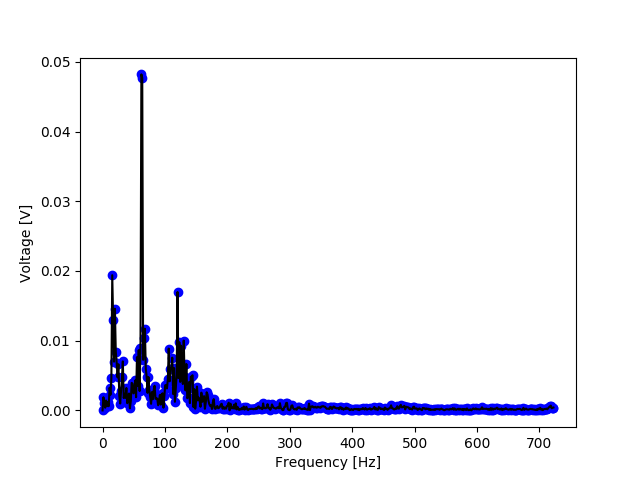
\includegraphics[width=0.7\textwidth]{DSP/Figs/3000_rpm_1khz_ok.png}
    %     \label{figure:spectrum}
    % \end{figure} 
    
 
    
    \section{Určení převodní konstanty}
        Z akcelerometru a AD převodníku získáváme údaj odpovídající pouze napětí. Pro jeho převod do jednotek odpovídajících zrychlení  – $\mathrm{m\,s^{-2}}$ nebo $g$ je třeba nalézt převodní konstantu.\\
        K tomuto úkolu byl využit referenční elektrodynamický budič vibrací (tzv. „shaker“) a přístrojový zesilovač NEXUS Conditioning amplifier s jednoosým přesným piezoelektrickým akcelerometrem s rozsahem 5000 $g$ \cite{manual:2}. Při použití obou akcelerometrů pro buzení motoru 400 Hz byla odečtena naměřená hodnota akcelerace na přípravku NEXUS a podle změřené efektivní hodnoty na použitém akcelerometru ADXL1002 vypočtena převodní konstanta.
        
        \begin{figure} [!h]
            \centering
            \caption{Přípravek NEXUS. Převzato z \cite{manual:2}.}
            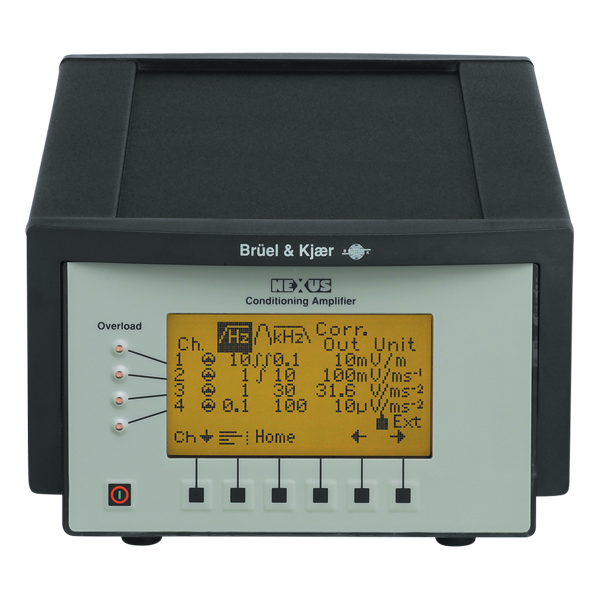
\includegraphics[width=0.5\textwidth]{DSP/Figs/nexus.png}
        \end{figure}       
        \begin{figure} [!t]
            \centering
            \caption{Výpočet převodní konstanty v laboratoři.}
            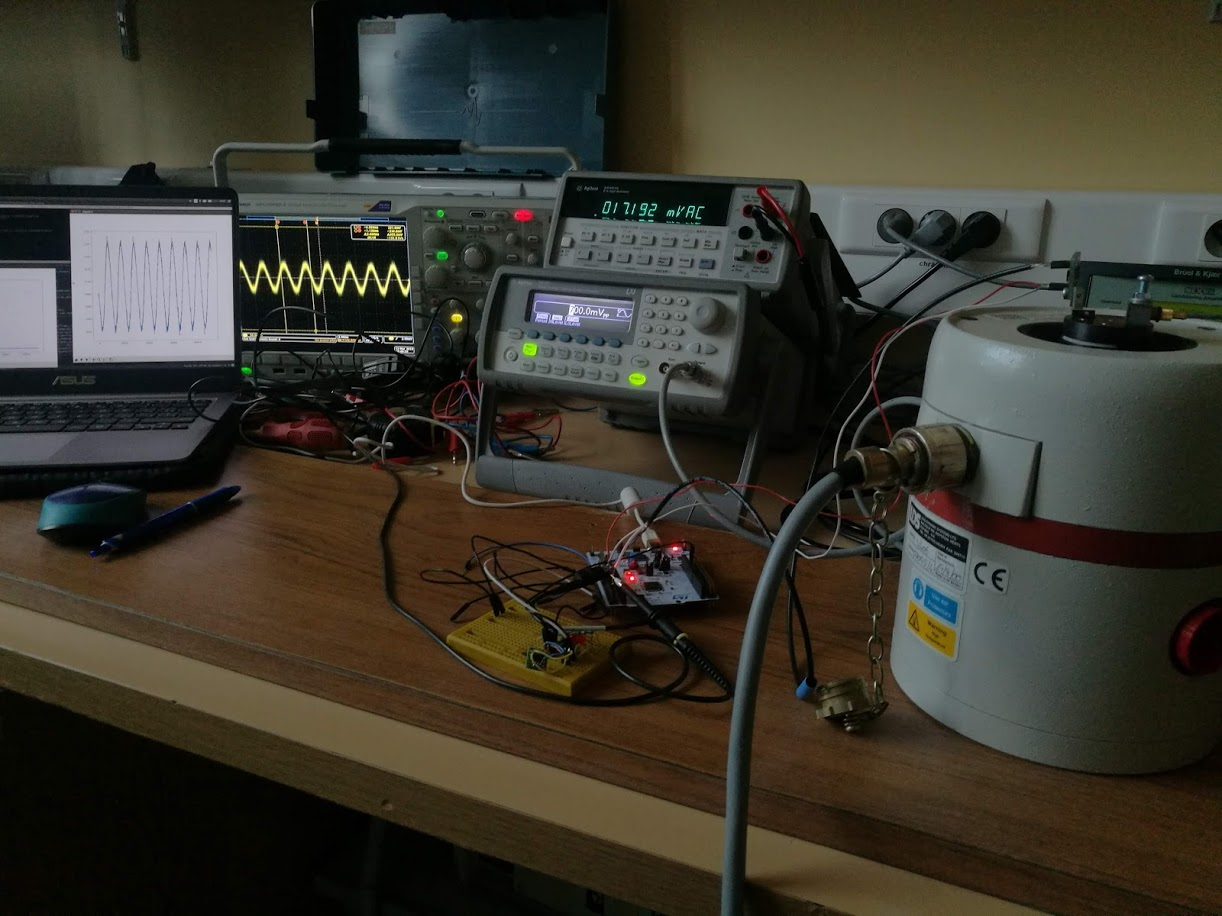
\includegraphics[width=\textwidth]{DSP/Figs/prakticka_zkouska.jpg}
        \end{figure} 
        
        
        
        

% ZDROJE 
% https://www.sczl.cz/download/download/2011-boretice/13-zkl-kotlan-vady-lozisek.pdf

% [55] S. G. Braun, Ed., Encyclopedia of Vibration. Elsevier, 2001.


% Kurtosis ratio
% J. Vass, R. Šmíd, R.B. Randall, “Avoidance of speckle noise in laser vibrometry by
% the use of kurtosis ratio: Application to mechanical fault diagnostics,” Mechanical
% Systems and Signal Processing, vol. 22, p. 647–671, 2008.
    
%CHECK ~
%CHECK red
%CHECK ...